% Appendix --- category-count (cardinality) tuning and reproducibility.
% The cardinality curve transforms the base macro F1 into an adjustable
% operating point; the figure is the real winner_cardinality_curve.png.
\appendix
\section{Ajuste del número de categorías: calidad vs.\ cobertura}
\label{app:cardinality}

Una decisión de despliegue prácticamente relevante es a cuántas
categorías de cultivo comprometerse. El ensamble final clasifica las 18
clases de PASTIS-R, pero seis cultivos minoritarios con fenología ambigua
arrastran a la baja el F1 macro global. La curva de cardinalidad responde
a una pregunta de negocio concreta: si el sistema se compromete solo a
los $K$ cultivos mejor resueltos, ¿qué calidad media se alcanza y qué
fracción de parcelas reales se cubre?

La metodología es honesta: el ranking de qué clase descartar se
determina sobre probabilidades out-of-fold del conjunto de entrenamiento,
y la métrica se mide sobre el fold de prueba retenido restringido a las
clases conservadas, de modo que la mejora no es un artefacto de selección
post-hoc. La Figura~\ref{fig:cardinality} muestra la curva completa.

\begin{figure}[htbp]
    \centering
    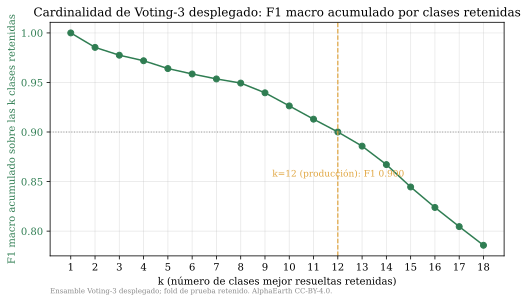
\includegraphics[width=0.9\columnwidth]
      {figures/us-070/cardinality_curve_es.png}
    \caption{Curva de cardinalidad del modelo Voting-3 desplegado.
    El codo alrededor de $K=8$--$9$ marca el equilibrio óptimo entre
    calidad y cobertura para la mayoría de los casos de uso.}
    \label{fig:cardinality}
\end{figure}
% src(figure): reports/voting_new/cardinalidad.json (Voting-3 desplegado)
% src(curve data): reports/voting_new/cardinalidad.json ["new"]:
%   F1 macro acumulado por K (K=18 0.786; K=12 0.900; K=9 0.940; K=8 0.949)

La curva arroja puntos de operación concretos (F1 macro acumulado por $K$
y la fracción de parcelas reales cubierta). En cardinalidad plena
($K=18$) el modelo Voting-3 desplegado alcanza un F1 macro de 0.786 sobre
el 100\% de las parcelas. Reducir a los 12 cultivos mejor resueltos eleva
el F1 macro a 0.900 cubriendo aún alrededor del 90\% de las parcelas
reales --- el punto de operación de producción recomendado, justo donde
la calidad cruza el umbral de 0.90; el modo de alta precisión ($K=9$)
alcanza un F1 macro de 0.940 con cerca del 82\% de cobertura; y un modo
de máxima confianza en $K=8$ alcanza un F1 macro de 0.949 sobre cerca del
80\% de las parcelas. El codo se sitúa alrededor de $K=8$--$9$, el
equilibrio óptimo entre calidad y cobertura para la mayoría de los casos
de uso. No se requiere reentrenamiento: el ensamble ya produce
probabilidades por clase, de modo que el umbral de categorías se aplica
dinámicamente en producción.

\section{Mezcla por vecindad espacial: un resultado nulo}
\label{app:neighbourhood}
También probamos si mezclar convexamente la posterior del campeón de cada
parcela con la posterior media de sus $k$ vecinos espaciales (centroide
$k$-NN en EPSG:2154, solo posteriors de vecinos, sin fuga de verdad de
terreno) mejora el F1 macro en el fold de prueba retenido. No lo hace: en
el espacio de etiquetas \texttt{france-9} el cambio es de $+0.0002$ de F1
macro en el mejor de los casos, dentro del ruido, y el espacio de 18
clases se mueve a lo sumo unas pocas milésimas antes de degradarse a
medida que crece el peso de la mezcla. Lo reportamos como un resultado
nulo honesto: el contexto espacial que la mezcla por vecindad añadiría ya
lo absorbe el embedding anual de AlphaEarth~\cite{brown2025alphaearth},
que codifica el contexto regional a nivel de parcela, de modo que un
término explícito de vecindad es redundante.
% src: reports/ensemble/metrics/ec_neighborhood_result.json
% (champion france9 0.9121; alpha sweep delta_f1_macro_france9 ~ +/-0.002, noise)

\section{Artefactos de reproducibilidad}
\label{app:repro}

Cada resultado cuantitativo está anclado a un artefacto versionado:

\begin{itemize}[leftmargin=*]
    \item Segmentación individual (fold-5):
    \texttt{reports/segmentation/metrics/model\_comparison\_fold5.csv}.
    \item Ensambles:
    \texttt{reports/ensemble/us043\_farslip\_summary.json} y
    \texttt{reports/ensemble/metrics/comparison\_us040.csv}.
    \item Espacio de características de FarSLIP:
    \texttt{reports/farslip/metrics/us037\_farslip\_fiel\_vs\_alphaearth.csv}.
    \item Transferencia Francia$\rightarrow$Cataluña:
    \texttt{reports/segmentation/sen4agrinet\_transfer\_result.json}.
    \item Conjuntos de datos (DVC): \texttt{data/sen4agrinet.dvc},
    \texttt{data/transfer/eurocropsml.dvc}.
\end{itemize}
